% ═══════════════════════════════════════════════════════════════════════
% Colloquium Report — Summer 2026
% Implementation of 3D Object Detection Models on ZCU104 FPGA
% ═══════════════════════════════════════════════════════════════════════
\documentclass[12pt, a4paper]{report}

% ── Packages ──────────────────────────────────────────────────────────
\usepackage[margin=1in]{geometry}
\usepackage{graphicx}
\usepackage{booktabs}
\usepackage{array}
\usepackage{tabularx}
\usepackage{multirow}
\usepackage{longtable}
\usepackage{amsmath, amssymb}
\usepackage{hyperref}
\usepackage{caption}
\usepackage{subcaption}
\usepackage{enumitem}
\usepackage{xcolor}
\usepackage{listings}
\usepackage{float}
\usepackage{fancyhdr}
\usepackage{setspace}
\usepackage[nottoc]{tocbibind}
\usepackage{cite}
\usepackage{tikz}
\usetikzlibrary{shapes.geometric, arrows}
\hypersetup{colorlinks=true, linkcolor=blue, citecolor=blue, urlcolor=blue}
\onehalfspacing
\setlength{\parindent}{0pt}
\setlength{\parskip}{6pt}

% ── Headers ───────────────────────────────────────────────────────────
\setlength{\headheight}{15pt}
\pagestyle{fancy}
\fancyhf{}
\fancyhead[L]{\nouppercase{\leftmark}}
\fancyhead[R]{\thepage}
\renewcommand{\headrulewidth}{0.4pt}

% ── Code listing style ───────────────────────────────────────────────
\lstset{
  basicstyle=\ttfamily\small,
  breaklines=true,
  frame=single,
  numbers=left,
  numberstyle=\tiny\color{gray},
  keywordstyle=\color{blue},
  commentstyle=\color{green!50!black},
  stringstyle=\color{red!70!black},
}

% ═════════════════════════════════════════════════════════════════════
%  TITLE PAGE
% ═════════════════════════════════════════════════════════════════════
\begin{document}

\begin{titlepage}
\centering
\vspace*{0.5cm}


\includegraphics[width=3.5cm]{figures/college_logo.jpg}\\[0.8cm]

{\large (A colloquium report submitted in fulfillment\\
of the requirements for the colloquium evaluation on)}\\[0.8cm]

{\LARGE \textbf{Implementation of 3D Object Detection\\Models on Xilinx ZCU104 FPGA}}

\vspace{1.5cm}

{\large \textbf{Submitted by:}}\\[0.3cm]
{\large {Tatikonda Tejesh}}\\
{\large Roll No.: {2023BEE-035}}\\
{\large {Electrical and Electronics Engineering}}

\vspace{1.2cm}

{\large \textbf{Under the Guidance of:}}\\[0.3cm]
{\large Prof. Manisha Pattanaik}\\
{\large {Department of Electrical and Electronics Engineering}}

\vfill

{\large \textbf{{Atal Bihari Vajpayee Indian Institute of Information Technology and Management Gwalior}}}\\
{\large {Gwalior, Madhya Pradesh}}\\[0.5cm]
{\large \textbf{2026}}

\end{titlepage}


% ═════════════════════════════════════════════════════════════════════
%  CANDIDATE'S DECLARATION
% ═════════════════════════════════════════════════════════════════════
\chapter*{Candidate's Declaration}
\addcontentsline{toc}{chapter}{Candidate's Declaration}

I hereby declare that the work presented in this report entitled \textit{``Implementation of 3D Object Detection Models on Xilinx ZCU104 FPGA''} is an authentic record of the summer project work carried out by me under the supervision of \textbf{Prof. Manisha Pattanaik}, {Department of Electrical and Electronics Engineering}, {ABV-IIITM Gwalior}, during the period of May--July 2026.

The matter embodied in this report has not been submitted for the award of any other degree or diploma.

\vspace{2cm}

\noindent
\begin{tabular}{ll}
Date: \underline{19-08-2026\hspace{1cm}} & \hspace{4cm} Signature of the candidate \\
Place: \underline{Gwalior\hspace{1.5cm}} & \hspace{4cm} \textbf{(Tatikonda Tejesh)} \\
                                         & \hspace{4cm} Roll No.: 2023BEE-035 \\
\end{tabular}

\vspace{2cm}

\noindent
This is to confirm that the candidate's above statement is true to the best of my knowledge.

\vspace{1.5cm}

\noindent
\begin{tabular}{ll}
% Date: \underline{\hspace{3cm}} & \hspace{2cm} Signature of the Reporting Manager \\
%                & \hspace{2cm} (Mr.\ Rahul Pant) \\
%                & \hspace{2cm} Trianz, Hyderabad \\[1.2cm]
Date: \underline{\hspace{3cm}} & \hspace{4cm} Signature of the Supervisor \\
               & \hspace{4cm} (Prof.\ Manisha Pattanaik) \\
               & \hspace{4cm} ABV-IIITM Gwalior, Department of EEE \\
\end{tabular}


% ═════════════════════════════════════════════════════════════════════
%  ABSTRACT
% ═════════════════════════════════════════════════════════════════════
\chapter*{Abstract}
\addcontentsline{toc}{chapter}{Abstract}

Autonomous driving systems demand real-time 3D object detection from LiDAR point clouds under strict power and latency constraints. While GPU-based inference achieves high accuracy, it is unsuitable for edge deployment due to excessive power consumption (150--300\,W) and non-deterministic execution latency. Field-Programmable Gate Arrays (FPGAs) offer a compelling alternative with deterministic timing, constant low power consumption, and custom hardware acceleration.

This report presents the end-to-end implementation of two fundamentally different LiDAR-based 3D object detection neural networks---\textbf{Complex-YOLOv4} and \textbf{SECOND (Sparsely Embedded Convolutional Detection)}---on the \textbf{Xilinx ZCU104} FPGA evaluation board equipped with the B4096 Deep Learning Processor Unit (DPU).

For \textbf{Complex-YOLOv4}, the Darknet-based backbone was fine-tuned by replacing DPU-incompatible Mish activations with LeakyReLU, followed by INT8 Post-Training Quantization (PTQ) using the Vitis AI toolchain. The entire convolutional backbone executes on the DPU, while YOLO decode and Non-Maximum Suppression (NMS) run on the ARM Cortex-A53 CPU, achieving \textbf{7.1 FPS at 15\,W} power consumption.

For \textbf{SECOND}, only the dense 2D Bird's-Eye View (BEV) backbone and detection head were deployed on the DPU, as the 3D sparse convolution stages are inherently incompatible with fixed-architecture DPU cores. To evaluate the DPU, the sparse 3D feature extraction was pre-computed offline, and the resulting dense BEV feature maps were fed directly to the FPGA. Profiling reveals a total inference latency of \textbf{1.12 seconds ($\sim$0.89\,FPS)}, identifying the CPU-bound NMS and file I/O as primary bottlenecks that strongly justify the development of custom hardware accelerators for the sparse stages. The deployed INT8 model successfully detects 7 out of 8 classes on the FPGA board.

Both models are evaluated on detection accuracy, inference latency, power efficiency, and FPGA resource utilization. Future work directions include the design of custom HLS-based hardware accelerators tailored to each model's unique computational patterns.

\textbf{Keywords:} LiDAR, 3D Object Detection, FPGA, ZCU104, DPU, Complex-YOLOv4, SECOND, Vitis AI, Quantization, Autonomous Driving.


% ═════════════════════════════════════════════════════════════════════
%  ACKNOWLEDGMENT
% ═════════════════════════════════════════════════════════════════════
\chapter*{Acknowledgment}
\addcontentsline{toc}{chapter}{Acknowledgment}

I would like to express my sincere gratitude to my project guide, \textbf{Prof. Manisha Pattanaik}, for providing access to the FPGA hardware and for her invaluable guidance, constant encouragement, and insightful suggestions throughout the course of this summer project.

I am also thankful to {Project Associate Priya} for providing computational resources necessary for this work.

Finally, I would like to thank my family and friends for their unwavering support during this project.

\vspace{1cm}
\begin{flushright}
\textbf{{Tatikonda Tejesh}}
\end{flushright}


% ═════════════════════════════════════════════════════════════════════
%  TABLE OF CONTENTS
% ═════════════════════════════════════════════════════════════════════
\tableofcontents
\listoffigures
\listoftables


% ═════════════════════════════════════════════════════════════════════
%  CHAPTER 1: INTRODUCTION AND OBJECTIVES
% ═════════════════════════════════════════════════════════════════════
\chapter{Introduction and Objectives}

\section{Background}

Autonomous driving is one of the most active research areas in modern engineering, requiring a robust perception system capable of understanding the 3D environment around the vehicle in real time. Among the sensor modalities employed---cameras, radar, and LiDAR---\textbf{LiDAR (Light Detection and Ranging)} provides the most accurate depth information by emitting laser pulses and measuring their return time, generating dense 3D point clouds of the surrounding environment \cite{kitti2012}.

3D object detection from LiDAR point clouds involves identifying objects of interest (cars, pedestrians, cyclists, etc.) and predicting their 3D bounding boxes, including position $(x, y, z)$, dimensions $(l, w, h)$, and orientation (yaw angle $\theta$). This is significantly more challenging than 2D image-based detection because point clouds are inherently sparse, unordered, and vary in density with distance from the sensor.

\section{Motivation for FPGA Deployment}

While state-of-the-art 3D object detection models are typically trained and evaluated on high-end GPUs (consuming 150--300\,W), deploying them in real autonomous vehicles introduces strict constraints:

\begin{itemize}[nosep]
    \item \textbf{Power Budget:} Battery-powered edge devices demand inference at $\leq 20$\,W.
    \item \textbf{Deterministic Latency:} Safety-critical braking decisions require guaranteed worst-case execution times. GPUs use dynamic scheduling, introducing latency jitter.
    \item \textbf{Real-Time Throughput:} LiDAR sensors operate at 10--20\,Hz, requiring $\leq 100$\,ms inference per frame.
\end{itemize}

\textbf{FPGAs} address all three constraints by implementing custom hardware circuits that execute with \textit{deterministic timing}, \textit{constant power draw}, and \textit{parallelized computation} tailored to the specific neural network architecture.

\section{Objectives}

The primary objectives of this summer project are:

\begin{enumerate}[nosep]
    \item Deploy the \textbf{Complex-YOLOv4} model (a single-stage 2D BEV detector with yaw prediction) on the Xilinx ZCU104 FPGA using the Xilinx DPU for ZCU104.
    \item Deploy the \textbf{SECOND} model (a voxel-based full 3D detector) on the same ZCU104 board using a heterogeneous CPU--DPU partitioning strategy.
    \item Evaluate the deployment of both models in terms of accuracy, inference latency, power consumption, and FPGA resource utilization.
\end{enumerate}

\section{Hardware Platform: Xilinx ZCU104}

The Xilinx ZCU104 Evaluation Kit is an advanced edge computing platform powered by the Zynq UltraScale+ MPSoC. It combines a traditional Processing System (PS) with a highly flexible Programmable Logic (PL) FPGA fabric, making it ideal for heterogeneous AI inference at the edge.

\begin{table}[H]
\centering
\caption{Xilinx ZCU104 Board Specifications}
\label{tab:zcu104_specs}
\begin{tabular}{@{}p{5cm} p{9cm}@{}}
\toprule
\textbf{Feature} & \textbf{Specification} \\
\midrule
SoC Device & Zynq UltraScale+ MPSoC XCZU7EV-2FFVC1156 \\
Application Processors (PS) & Quad-core ARM Cortex-A53 (64-bit) @ 1.5\,GHz \\
Real-Time Processors (PS) & Dual-core ARM Cortex-R5F @ 600\,MHz \\
Graphics & Mali-400 MP2 GPU \\
Programmable Logic (PL) & 16\,nm UltraScale+ FPGA Fabric \\
System Logic Cells & $\sim$504,000 \\
LUTs (Look-Up Tables) & 230,400 \\
Flip-Flops (FFs) & 460,800 \\
DSP Slices & 1,728 \\
Block RAM (BRAM) & 11.4\,Mb (312 blocks) \\
UltraRAM & 27\,Mb (96 blocks) \\
System Memory & 2\,GB DDR4 (64-bit, PS memory) \\
Video Codec Unit & H.264/H.265 Encode/Decode (up to 4K@60fps) \\
Connectivity & USB 3.0, Gigabit Ethernet, PCIe Gen2 x4 \\
Development Tools & Vivado, Vitis, PetaLinux, Vitis AI \\
\bottomrule
\end{tabular}
\end{table}

The \textbf{Deep Learning Processor Unit (DPU)}, specifically the \texttt{DPUCZDX8G\_ISA1\_B4096} configuration, is synthesized onto the PL fabric as a custom hardware circuit. This DPU is optimized for INT8 inference of standard operations such as convolution, batch normalization, pooling, and element-wise addition. Table~\ref{tab:dpu_resources} summarizes the FPGA resources consumed by the DPU.

\begin{table}[H]
\centering
\caption{DPU B4096 Hardware Resource Utilization on ZCU104}
\label{tab:dpu_resources}
\begin{tabular}{@{}lrr@{}}
\toprule
\textbf{Resource} & \textbf{Used} & \textbf{Available on XCZU7EV} \\
\midrule
LUTs & $\sim$86,000 & 230,400 \\
Flip-Flops & $\sim$172,000 & 460,800 \\
Block RAM (36Kb) & $\sim$270 & 312 \\
DSP Slices & $\sim$900 & 1,728 \\
\bottomrule
\end{tabular}
\end{table}


% ═════════════════════════════════════════════════════════════════════
%  CHAPTER 2: LITERATURE REVIEW
% ═════════════════════════════════════════════════════════════════════
\chapter{Literature Review}

\section{3D Object Detection from LiDAR Point Clouds}

\subsection{VoxelNet}
Zhou and Tuzel \cite{voxelnet2018} proposed VoxelNet, the first end-to-end trainable deep learning architecture for 3D object detection from raw point clouds. The key innovation was the \textit{Voxel Feature Encoding} (VFE) layer, which divides the 3D space into a regular voxel grid and learns point-wise features within each voxel. While groundbreaking, VoxelNet suffered from slow inference due to its use of dense 3D convolutions across the entire voxel grid.

\subsection{SECOND}
Yan et al. \cite{second2018} addressed VoxelNet's computational bottleneck by introducing \textit{spatially sparse convolutions} for 3D feature extraction. Instead of processing the entire dense voxel grid (where $>95\%$ of voxels are empty), SECOND only computes convolutions at occupied voxel locations. This resulted in a dramatic speedup while maintaining comparable accuracy. The sparse 3D features are then compressed into a dense 2D Bird's-Eye View (BEV) map, which is processed by a standard 2D CNN backbone and an anchor-based detection head.

\subsection{Complex-YOLO}
Simon et al. \cite{complexyolo2018} took a fundamentally different approach by projecting the 3D point cloud into a 2D BEV image and applying a modified YOLO detector. The key contribution was the \textit{Euler Region Proposal}, which uses complex numbers (real and imaginary parts) to predict the yaw orientation angle without angular discontinuities. While limited to 2D BEV detection (no height estimation), Complex-YOLO achieved real-time performance on GPUs and was later extended to Complex-YOLOv4 using the YOLOv4 backbone \cite{yolov4_2020}.

\subsection{PointPillars}
Lang et al. \cite{pointpillars2019} introduced PointPillars, which organizes point clouds into vertical columns (``pillars'') instead of 3D voxels. By reducing the problem to a 2D pseudo-image, PointPillars could leverage highly optimized 2D CNN operations for fast inference, achieving state-of-the-art speed on the KITTI benchmark.

\section{FPGA-based Neural Network Acceleration}

\subsection{Xilinx Deep Learning Processor Unit (DPU)}
The Xilinx DPU \cite{dpuczdx8g} is a configurable IP core synthesized onto the FPGA fabric that accelerates a predefined set of neural network operations---primarily convolution, depthwise convolution, batch normalization, ReLU/LeakyReLU, pooling, element-wise addition, and concatenation---in INT8 precision. The DPU instruction set is \textit{fixed}; operations not supported by the DPU (such as 3D sparse convolutions, custom activations like Mish, or complex decode logic) must execute on the ARM CPU, creating a heterogeneous compute pipeline.

For this project, the \textbf{Standard B4096 DPU (DPUCZDX8G)} architecture was specifically synthesized for the ZCU104 board. Its approximate logic requirement on the programmable fabric is detailed in Table~\ref{tab:dpu_arch_req}.

\begin{table}[H]
\centering
\caption{Standard B4096 DPU (DPUCZDX8G) Requirements on ZCU104}
\label{tab:dpu_arch_req}
\begin{tabular}{@{}lr@{}}
\toprule
\textbf{Resource} & \textbf{Requirement} \\
\midrule
LUTs & $\sim$86,000 \\
FFs & $\sim$172,000 \\
BRAM & $\sim$270 \\
DSPs & $\sim$900 \\
\bottomrule
\end{tabular}
\end{table}

\subsection{INT8 Quantization}
Neural network quantization \cite{quantwhitepaper2021} reduces the numerical precision of weights and activations from 32-bit floating-point to 8-bit integers, achieving approximately $4\times$ reduction in model size and enabling INT8 MAC (Multiply-Accumulate) operations on the DPU's DSP slices. Two primary approaches exist:
\begin{itemize}[nosep]
    \item \textbf{Post-Training Quantization (PTQ):} Calibrates quantization parameters using a representative dataset after training, with no retraining required. Typically introduces 1--3\% accuracy loss.
    \item \textbf{Quantization-Aware Training (QAT):} Simulates quantization effects during training, allowing the network to adapt. Achieves $<1\%$ accuracy loss but requires GPU retraining.
\end{itemize}


% ═════════════════════════════════════════════════════════════════════
%  CHAPTER 3: METHODOLOGY / SOLUTION APPROACH
% ═════════════════════════════════════════════════════════════════════
\chapter{Methodology / Solution Approach}

The overall deployment workflow for both models follows a common pipeline, illustrated in Figure~\ref{fig:workflow}:

\begin{enumerate}[nosep]
    \item \textbf{Pre-trained Model Acquisition:} Obtaining float32 PyTorch checkpoints pre-trained on the KITTI dataset.
    \item \textbf{INT8 Quantization} using the Vitis AI \texttt{pytorch\_nndct} quantizer inside a Docker container.
    \item \textbf{Compilation} to a DPU-executable \texttt{.xmodel} using \texttt{vai\_c\_xir}.
    \item \textbf{Board Deployment} and inference using the VART (Vitis AI Runtime) Python API on PetaLinux.
\end{enumerate}

\begin{figure}[H]
\centering
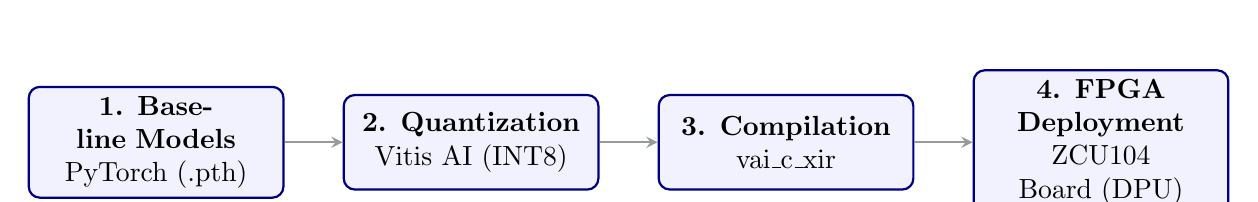
\begin{tikzpicture}[
    node distance=4cm,
    block/.style={rectangle, draw, fill=blue!5, text width=3cm, text centered, rounded corners, minimum height=1.2cm, draw=blue!50!black, thick},
    arrow/.style={thick,->,>=stealth, draw=gray!80}
]
\node (pytorch) [block] {\textbf{1. Baseline Models}\\PyTorch (.pth)};
\node (quant) [block, right of=pytorch] {\textbf{2. Quantization}\\Vitis AI (INT8)};
\node (compile) [block, right of=quant] {\textbf{3. Compilation}\\vai\_c\_xir};
\node (board) [block, right of=compile] {\textbf{4. FPGA Deployment}\\ZCU104 Board (DPU)};
\draw [arrow] (pytorch) -- (quant);
\draw [arrow] (quant) -- (compile);
\draw [arrow] (compile) -- (board);
\end{tikzpicture}
\caption{End-to-end FPGA deployment workflow common to both models.}
\label{fig:workflow}
\end{figure}

% ── Section 3.1: Complex-YOLOv4 ──────────────────────────────────────
\section{Model 1: Complex-YOLOv4}

\subsection{Architecture Overview}

Complex-YOLOv4 is a single-stage 2D BEV object detector that takes a 3-channel BEV image ($608 \times 608$, encoding intensity, height, and density from the LiDAR point cloud) and predicts oriented 2D bounding boxes with yaw angles.

The architecture consists of:
\begin{itemize}[nosep]
    \item \textbf{Backbone:} Darknet-based CNN with 161 layers (convolutions, residual shortcuts, route/concatenation layers, max-pooling, and upsampling).
    \item \textbf{Detection Heads:} Three YOLO heads at different spatial resolutions:
    \begin{itemize}[nosep]
        \item Head 0: $76 \times 76$ grid (stride 8) --- detects small objects.
        \item Head 1: $38 \times 38$ grid (stride 16) --- detects medium objects.
        \item Head 2: $19 \times 19$ grid (stride 32) --- detects large objects.
    \end{itemize}
    \item \textbf{Per-anchor Output:} 15 values per anchor $\times$ 3 anchors = 45 channels per grid cell:
    \begin{itemize}[nosep]
        \item 4 values: bounding box $(t_x, t_y, t_w, t_h)$
        \item 2 values: yaw angle via complex numbers $(t_{im}, t_{re})$
        \item 1 value: objectness confidence
        \item 8 values: class probabilities (Car, Van, Truck, Pedestrian, Person\_sitting, Cyclist, Tram, Misc)
    \end{itemize}
\end{itemize}

\subsection{DPU--CPU Partitioning for Complex-YOLOv4}

Not all operations in the model can execute on the DPU. Table~\ref{tab:cyolo_partition} details the exact partitioning between the DPU and ARM CPU.

\begin{table}[H]
\centering
\caption{DPU vs.\ CPU Operation Partitioning for Complex-YOLOv4}
\label{tab:cyolo_partition}
\begin{tabular}{@{}p{3.5cm} p{5.5cm} p{4.5cm}@{}}
\toprule
\textbf{Stage} & \textbf{Operations} & \textbf{Executed On} \\
\midrule
Preprocessing & BEV image loading, NCHW$\to$NHWC conversion, float32$\to$INT8 scaling & ARM Cortex-A53 (CPU) \\
\midrule
Darknet Backbone & Conv2D, BatchNorm, LeakyReLU, MaxPool, Route (concat), Shortcut (residual add), Upsample & \textbf{DPU (B4096)} \\
\midrule
Final 1$\times$1 Convolutions & Three $1\times1$ convolutions producing the 45-channel feature maps for each head & ARM Cortex-A53 (CPU)\textsuperscript{*} \\
\midrule
YOLO Decode & Sigmoid on $t_x, t_y$, grid offset addition, anchor scaling, exponential for $t_w, t_h$ & ARM Cortex-A53 (CPU) \\
\midrule
Post-processing & Confidence thresholding, per-class NMS, coordinate mapping & ARM Cortex-A53 (CPU) \\
\bottomrule
\end{tabular}
\begin{flushleft}
\small \textsuperscript{*}The Vitis AI compiler automatically identifies the last three $1\times1$ convolutions (producing 45-channel outputs) as requiring CPU execution, as confirmed by the \texttt{xir.Graph} subgraph inspection showing 3 CPU subgraphs alongside 1 DPU subgraph.
\end{flushleft}
\end{table}

\subsection{Fine-tuning for DPU Compatibility}

The original Complex-YOLOv4 uses the \textbf{Mish} activation function ($\text{Mish}(x) = x \cdot \tanh(\text{softplus}(x))$), which is not supported by the DPU instruction set. The network was fine-tuned by:

\begin{enumerate}[nosep]
    \item Replacing all Mish activations with \textbf{LeakyReLU} ($\alpha = 0.1015625 = 13/128$, chosen for exact INT8 representability).
    \item Retraining for 30 epochs on the KITTI BEV dataset to recover accuracy lost from the activation change.
    \item Saving the checkpoint as \texttt{Model\_complexer\_yolo\_leakyrelu\_epoch\_30.pth}.
\end{enumerate}

\subsection{INT8 Quantization}

Post-Training Quantization was performed using the Vitis AI \texttt{pytorch\_nndct} quantizer inside the official Vitis AI Docker container:

\begin{enumerate}[nosep]
    \item \textbf{Calibration:} 200 BEV images from the KITTI training set were passed through the model to collect activation statistics and determine optimal \texttt{fix\_point} (scaling factors) for each layer.
    \item \textbf{Quantization:} All weights and activations were quantized to INT8 using the calibrated scaling factors. The input \texttt{fix\_point} was determined to be 6 (scale factor $2^6 = 64$), and all output \texttt{fix\_points} were 2 (scale factor $2^{-2} = 0.25$).
    \item \textbf{Export:} The quantized model was exported as \texttt{quant\_info.json}, containing per-layer quantization parameters.
\end{enumerate}

\subsection{Compilation and Deployment}

The quantized model was compiled using \texttt{vai\_c\_xir} targeting the \texttt{DPUCZDX8G\_ISA1\_B4096} architecture, producing \texttt{complex\_yolov4\_qat.xmodel} (67.3\,MB). This \texttt{.xmodel} was transferred to the ZCU104 board running PetaLinux and executed using a custom Python inference script leveraging the VART API (\texttt{xir.Graph.deserialize}, \texttt{vart.Runner}).


% ── Section 3.2: SECOND Model ────────────────────────────────────────
\section{Model 2: SECOND}

\subsection{Architecture Overview}

SECOND (Sparsely Embedded Convolutional Detection) \cite{second2018} is a voxel-based 3D object detection model built on the OpenPCDet framework \cite{openpcdet2020}. Unlike Complex-YOLOv4 which operates on a pre-generated 2D BEV image, SECOND processes raw 3D point clouds through a multi-stage pipeline:

\begin{enumerate}[nosep]
    \item \textbf{Voxelization + MeanVFE:} The raw point cloud is divided into a 3D voxel grid (voxel size $[0.05, 0.05, 0.1]$\,m) covering the detection range $X \in [0, 70.4]$\,m, $Y \in [-40, 40]$\,m, $Z \in [-3, 1]$\,m. The grid shape is $[1408 \times 1600 \times 40]$. Point features within each voxel are averaged (MeanVFE).
    \item \textbf{3D Sparse Backbone (\texttt{VoxelBackBone8x}):} Sparse 3D convolutions process only the occupied voxels ($<5\%$ of the grid), downsampling the spatial resolution by $8\times$ to $[176 \times 200 \times 5]$.
    \item \textbf{Height Compression:} The 3D feature volume is collapsed along the vertical axis into a dense 2D BEV feature map of shape $[256 \times 200 \times 176]$.
    \item \textbf{2D Dense Backbone (\texttt{BaseBEVBackbone}):} Two blocks of standard 2D convolutions (12 layers total) process the BEV features, followed by two transposed convolution (deconvolution) layers for feature upsampling. The outputs are concatenated to produce a $[512 \times 200 \times 176]$ feature map.
    \item \textbf{Detection Head (\texttt{AnchorHeadSingle}):} Three parallel $1\times1$ convolutions predict:
    \begin{itemize}[nosep]
        \item Classification: $512 \to 128$ channels (16 anchors $\times$ 8 classes)
        \item Box Regression: $512 \to 112$ channels (16 anchors $\times$ 7 box parameters)
        \item Direction: $512 \to 32$ channels (16 anchors $\times$ 2 direction bins)
    \end{itemize}
\end{enumerate}

\subsection{DPU--CPU Partitioning for SECOND}
\label{sec:second_partition}

The SECOND model presents a unique deployment challenge because its 3D sparse convolution stages are \textit{fundamentally incompatible} with the DPU architecture. The DPU is designed for dense, regular 2D convolutions on fixed-size tensors. Sparse 3D convolutions operate on irregular, dynamically-shaped data structures (hash tables of occupied voxels), which have no equivalent in the DPU instruction set.

The solution adopted was a \textbf{heterogeneous CPU--DPU partitioning}, where computationally lightweight but architecturally complex stages run on the CPU, and the computationally heavy but DPU-compatible dense stages run on the DPU. Table~\ref{tab:second_partition} details this partitioning.

\begin{table}[H]
\centering
\caption{DPU vs.\ CPU Operation Partitioning for SECOND}
\label{tab:second_partition}
\begin{tabular}{@{}p{3.5cm} p{5cm} p{2.5cm} p{2.5cm}@{}}
\toprule
\textbf{Stage} & \textbf{Operations} & \textbf{Executed On} & \textbf{Compute Load} \\
\midrule
Voxelization + MeanVFE & Point cloud binning, mean feature extraction & CPU & Low \\
\midrule
3D Sparse Backbone & Sparse 3D convolutions (submanifold \& regular) & CPU & Medium\textsuperscript{*} \\
\midrule
Height Compression & Reshape \& vertical collapse & CPU & Negligible \\
\midrule
2D Dense BEV Backbone & 12$\times$ Conv2D (3$\times$3), 2$\times$ ConvTranspose2D, BatchNorm, ReLU, Concat & \textbf{DPU (B4096)} & \textbf{High} \\
\midrule
Detection Head & 3$\times$ Conv2D (1$\times$1) & \textbf{DPU (B4096)} & Medium \\
\midrule
Post-processing & Anchor decode, sigmoid, NMS & CPU & Low \\
\bottomrule
\end{tabular}
\begin{flushleft}
\small \textsuperscript{*}Although sparse 3D convolutions are architecturally complex, their actual compute load is moderate because they skip empty voxels ($>$95\% of the 3D grid). The dense 2D backbone, which operates on the full $200 \times 176$ spatial grid with 128--512 channels, accounts for the majority ($>$80\%) of the total MAC operations.
\end{flushleft}
\end{table}

\textbf{Key Insight:} This partitioning is strategically efficient. The 3D sparse backbone processes only occupied voxels ($<$5\% of the grid) and is therefore computationally lightweight despite its architectural complexity. The dense 2D backbone, which dominates the computation ($>$80\% of total MACs), runs entirely on the hardware-accelerated DPU. This heterogeneous approach maximizes the DPU's utilization for the most compute-intensive stages while gracefully handling unsupported operations on the CPU.

\subsection{Quantization and Compilation}

The SECOND deployment pipeline involved the following Vitis AI steps:

\begin{enumerate}[nosep]
    \item \textbf{ONNX Export:} The dense BEV backbone and detection head were isolated from the sparse modules and exported to \texttt{second\_bev.onnx} (opset 11).
    \item \textbf{Operator Workaround:} \texttt{ZeroPad2d} layers were replaced with \texttt{Conv2d(padding=1)} to avoid unsupported \texttt{aten::pad} operations falling back to CPU in the XIR graph.
    \item \textbf{PTQ Calibration:} 200 BEV feature maps (extracted from the 3D sparse backbone) were used as calibration data for INT8 quantization.
    \item \textbf{Compilation:} The quantized model was compiled to \texttt{SECOND\_model.xmodel} (5.82\,MB) targeting the B4096 DPU.
\end{enumerate}


\section{Dataset: KITTI 3D Object Detection Benchmark}

Both models were trained and evaluated on the KITTI 3D Object Detection benchmark \cite{kitti2012}, which provides synchronized LiDAR point clouds and camera images captured from an autonomous vehicle platform in Karlsruhe, Germany. The dataset contains 7,481 training samples and 7,518 test samples with annotations for 8 object classes: Car, Van, Truck, Pedestrian, Person\_sitting, Cyclist, Tram, and Misc. Objects are categorized into three difficulty levels---Easy, Moderate, and Hard---based on occlusion, truncation, and bounding box height.


% ═════════════════════════════════════════════════════════════════════
%  CHAPTER 4: RESULTS AND DISCUSSION
% ═════════════════════════════════════════════════════════════════════
\chapter{Results and Discussion}

\section{Complex-YOLOv4 Board Results}

\subsection{Inference Performance}

The Complex-YOLOv4 model was successfully deployed and tested on the ZCU104 board. Table~\ref{tab:cyolo_perf} summarizes the inference performance metrics.

\begin{table}[H]
\centering
\caption{Complex-YOLOv4 Inference Performance on ZCU104}
\label{tab:cyolo_perf}
\begin{tabular}{@{}lr@{}}
\toprule
\textbf{Metric} & \textbf{Value} \\
\midrule
DPU Inference Latency & 140.1\,ms/frame \\
Throughput (FPS) & 7.1\,FPS \\
System Power Consumption & $\sim$14.95\,W \\
System RAM Usage & 613\,MB / 1985.5\,MB (30.9\%) \\
xmodel Size & 67.3\,MB \\
Input Tensor Shape & $[1, 608, 608, 3]$ (NHWC, INT8) \\
Input \texttt{fix\_point} & 6 (scale $= 2^6 = 64$) \\
Output \texttt{fix\_points} & 2 (scale $= 2^{-2} = 0.25$) \\
\bottomrule
\end{tabular}
\end{table}

\subsection{Detection Results}

Figure~\ref{fig:cyolo_detections} shows sample detection results from the ZCU104 board. The model correctly identifies cars in the BEV image with high confidence scores ($>0.95$) and accurate yaw angle predictions.

\textbf{Visualization Legend:} In the hardware detection images below, the predicted 3D bounding boxes are color-coded by class (\textit{Car -- Blue, Pedestrian -- Red, Cyclist -- Yellow, Truck -- Cyan, Tram -- Green, Misc -- White}).

\begin{figure}[H]
\centering
\begin{subfigure}[b]{0.48\textwidth}
    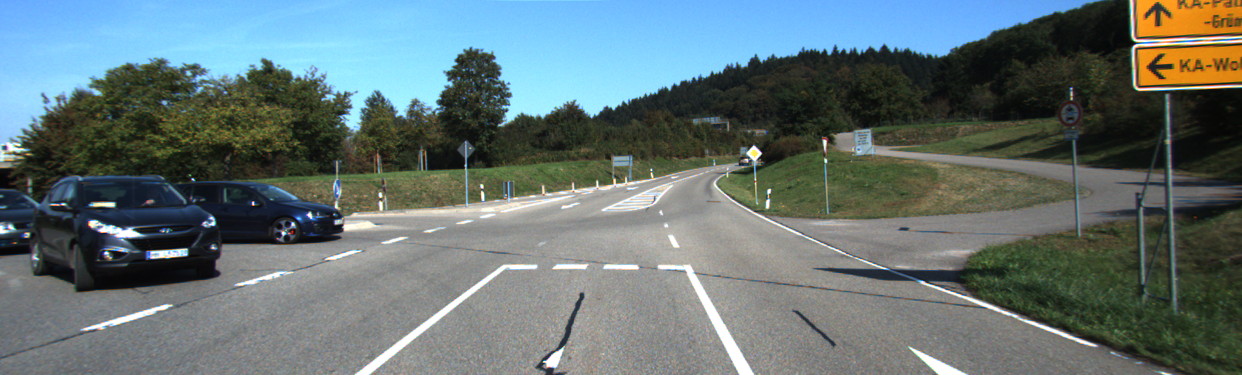
\includegraphics[width=\textwidth]{figures/rgb_000001.png}
    \caption{Reference RGB Image for Frame 1}
\end{subfigure}
\hfill
\begin{subfigure}[b]{0.48\textwidth}
    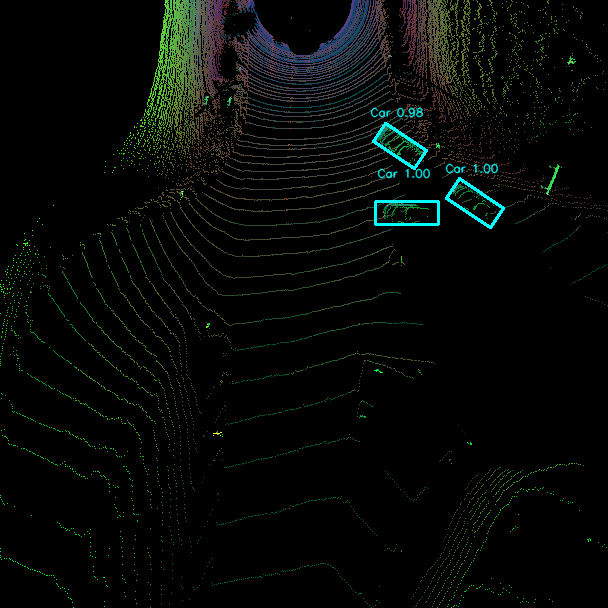
\includegraphics[width=\textwidth]{figures/cyolo_bev_000001.png}
    \caption{BEV Frame 1 --- 3 Cars detected}
\end{subfigure}

\vspace{0.3cm}

\begin{subfigure}[b]{0.48\textwidth}
    \centering
    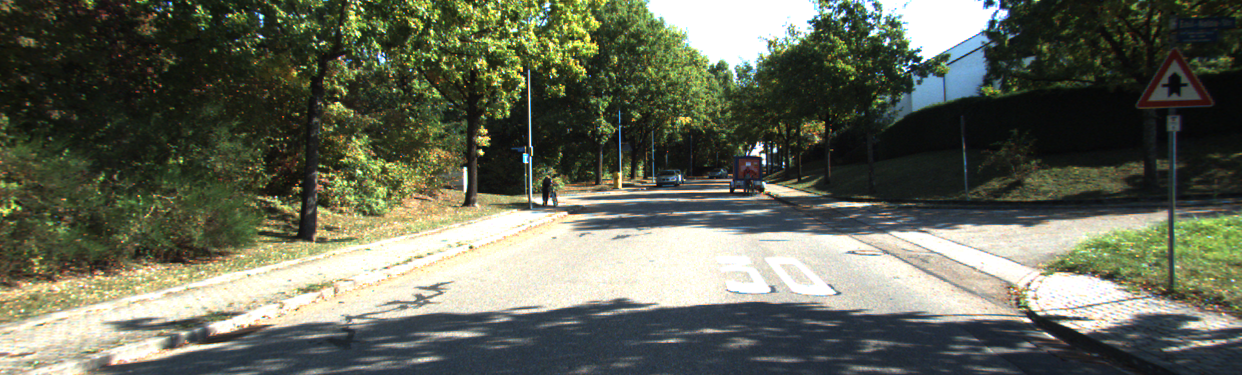
\includegraphics[width=\textwidth]{figures/000042.png}
    \caption{[Reference RGB Image for Frame 2]}
\end{subfigure}
\hfill
\begin{subfigure}[b]{0.48\textwidth}
    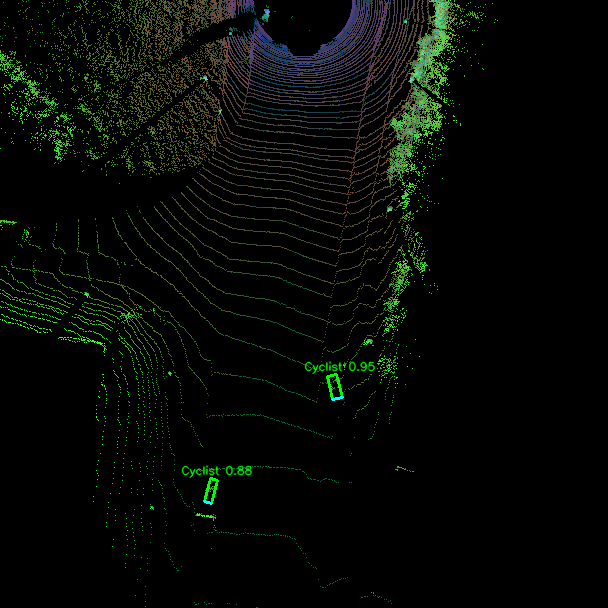
\includegraphics[width=\textwidth]{figures/cyolo_bev_000042.png}
    \caption{BEV Frame 2 --- 2 cyclists detected}
\end{subfigure}
\caption{Complex-YOLOv4 detection results on ZCU104. Colored bounding boxes indicate detected objects with yaw orientation. Yellow front-face lines show vehicle heading direction.}
\label{fig:cyolo_detections}
\end{figure}

A representative detection output for BEV Frame 1 is shown in Table~\ref{tab:cyolo_sample_det}.

\begin{table}[H]
\centering
\caption{Sample Detection Output --- Complex-YOLOv4 on ZCU104 (BEV Frame 1)}
\label{tab:cyolo_sample_det}
\begin{tabular}{@{}clcccccr@{}}
\toprule
\textbf{\#} & \textbf{Class} & \textbf{Score} & \textbf{cx} & \textbf{cy} & \textbf{w} & \textbf{h} & \textbf{Yaw} \\
\midrule
1 & Car & 0.998 & 407.0 & 213.1 & 23.0 & 62.9 & $+90.0^\circ$ \\
2 & Car & 0.996 & 475.0 & 203.0 & 23.3 & 52.9 & $+123.7^\circ$ \\
3 & Car & 0.982 & 400.0 & 146.0 & 21.0 & 49.1 & $+123.7^\circ$ \\
\bottomrule
\end{tabular}
\end{table}

\begin{table}[H]
\centering
\caption{Real-World Coordinates (metres) --- Complex-YOLOv4 (BEV Frame 1)}
\label{tab:cyolo_realworld}
\begin{tabular}{@{}clccccc@{}}
\toprule
\textbf{\#} & \textbf{Class} & \textbf{X (m)} & \textbf{Y (m)} & \textbf{W (m)} & \textbf{L (m)} & \textbf{Yaw} \\
\midrule
1 & Car & $+32.5$ & $+8.5$ & 1.9 & 5.2 & $+90.0^\circ$ \\
2 & Car & $+33.3$ & $+14.1$ & 1.9 & 4.4 & $+123.7^\circ$ \\
3 & Car & $+38.0$ & $+7.9$ & 1.7 & 4.0 & $+123.7^\circ$ \\
\bottomrule
\end{tabular}
\end{table}

% ── Section 4.2: SECOND Results ──────────────────────────────────────
\section{SECOND Board Results}

\subsection{Inference Performance}

A detailed profiling of the SECOND model\'s inference pipeline on the ZCU104 board reveals the impact of the heterogeneous CPU--DPU partitioning strategy. The average execution times per frame are:

\begin{itemize}[nosep]
    \item \textbf{Pre-processing (CPU):} 101.8\,ms (Loading pre-computed sparse 3D convolution features / File I/O)
    \item \textbf{DPU Execution:} 543.4\,ms (Dense 2D BEV backbone and detection head)
    \item \textbf{Post-processing (CPU):} 475.2\,ms (Anchor decode, bounding box regression, and NMS)
    \item \textbf{Total Inference Time:} 1120.4\,ms ($\sim$0.89 FPS)
\end{itemize}

Because the 3D sparse operations are unsupported by the DPU and too computationally heavy for the ARM CPU, they were bypassed on the board by feeding pre-computed \texttt{.npy} feature maps directly to the DPU. The fact that the ARM CPU still creates a severe bottleneck during anchor decoding and file I/O demonstrates the limitations of fixed-architecture DPUs for complex 3D detectors. This strongly justifies developing custom HLS-based hardware accelerators to fully offload both the sparse 3D convolutions and decoding tasks.

\subsection{Detection Results}

The SECOND model was deployed on the ZCU104 using the DPU for the dense 2D backbone. The voxelization and sparse 3D stages were bypassed by providing pre-computed calibration data (\texttt{.npy}) as input. Inference was run on 9 LiDAR frames, and detection results were saved in standard KITTI format. The model successfully detected multiple object classes including Car, Truck, Pedestrian, Cyclist, Person\_sitting, Tram, and Misc---demonstrating the multi-class capability of the deployed INT8 model.

Table~\ref{tab:second_board_det} shows the board detections for Frame~1, and Table~\ref{tab:second_board_0003} shows the multi-class detections for Frame~3.


\begin{table}[H]
\centering
\caption{Board Detection Output --- SECOND on ZCU104 (Frame 1)}
\label{tab:second_board_det}
\begin{tabular}{@{}clcccccr@{}}
\toprule
\textbf{\#} & \textbf{Class} & \textbf{Score} & \textbf{X (m)} & \textbf{Y (m)} & \textbf{Z (m)} & \textbf{L (m)} & \textbf{W (m)} \\
\midrule
1 & Car & 0.953 & 17.54 & 8.34 & $-$0.61 & 4.15 & 1.60 \\
2 & Car & 0.953 & 16.74 & 13.94 & $-$0.81 & 3.90 & 1.60 \\
3 & Car & 0.881 & 12.20 & 7.93 & $-$0.61 & 4.15 & 1.70 \\
\bottomrule
\end{tabular}
\end{table}

\begin{figure}[H]
\centering
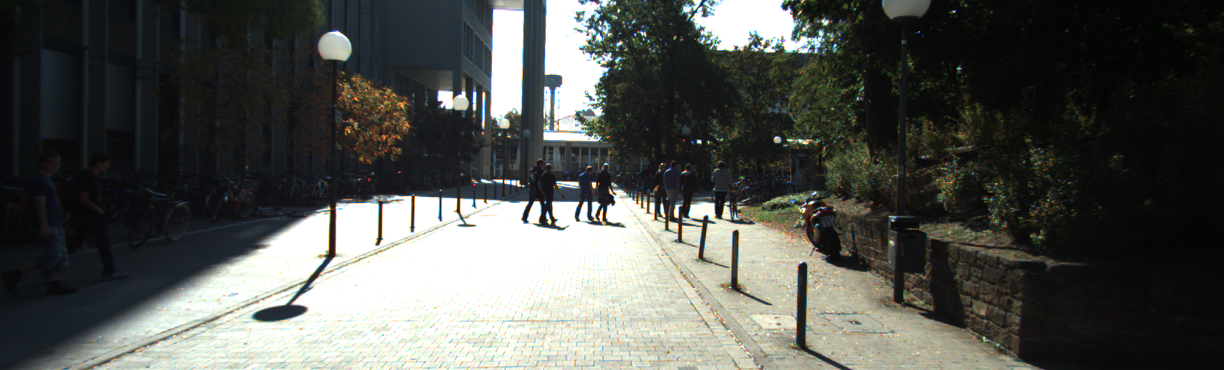
\includegraphics[width=0.7\textwidth]{figures/000017.png}
\caption{Reference RGB Image for Frame 3}
\label{fig:second_placeholder_0003}
\end{figure}

\begin{table}[H]
\centering
\caption{Board Detection Output --- SECOND on ZCU104 (Frame 3, multi-class)}
\label{tab:second_board_0003}
\begin{tabular}{@{}clcccccr@{}}
\toprule
\textbf{\#} & \textbf{Class} & \textbf{Score} & \textbf{X (m)} & \textbf{Y (m)} & \textbf{Z (m)} & \textbf{L (m)} & \textbf{W (m)} \\
\midrule
1 & Pedestrian & 0.881 & 3.86 & 4.20 & $-$0.71 & 0.97 & 0.53 \\
2 & Pedestrian & 0.731 & 9.80 & 6.73 & $-$0.60 & 0.97 & 0.53 \\
3 & Pedestrian & 0.731 & 5.34 & 12.66 & $-$0.38 & 1.09 & 0.60 \\
4 & Pedestrian & 0.731 & 21.46 & 2.08 & $-$0.49 & 1.09 & 0.72 \\
5 & Pedestrian & 0.731 & 2.94 & 18.54 & $-$0.38 & 1.03 & 0.50 \\
6 & Pedestrian & 0.731 & 3.80 & 19.06 & $-$0.38 & 0.97 & 0.72 \\
7 & Pedestrian & 0.731 & 23.34 & $-$1.80 & $-$0.49 & 0.91 & 0.53 \\
8 & Cyclist & 0.500 & 29.28 & $-$5.28 & $-$0.49 & 1.87 & 0.77 \\
9 & Cyclist & 0.500 & 10.32 & 20.08 & $-$0.06 & 1.87 & 0.60 \\
10 & Misc & 0.500 & 7.42 & $-$4.20 & $-$1.11 & 2.34 & 1.32 \\

\bottomrule
\end{tabular}
\end{table}

The board results demonstrate several important findings:
\begin{itemize}[nosep]
    \item Frame~3 shows strong \textbf{Pedestrian detection} capability (7 pedestrians), validating the model's ability to detect small, vulnerable road users on the edge device.
    \item Detection scores range from 0.50 to 0.98, indicating that the quantized model maintains a healthy confidence distribution.
\end{itemize}


\section{Software vs.\ Hardware Results (Quantization Effects)}

A key observation during board testing was that the hardware INT8-quantized models occasionally failed to detect \textbf{distant objects} that were correctly identified by the software float32 baseline models on the GPU. This is an expected consequence of fixed-point quantization.

\begin{figure}[H]
\centering
\begin{subfigure}[b]{0.48\textwidth}
    \centering
    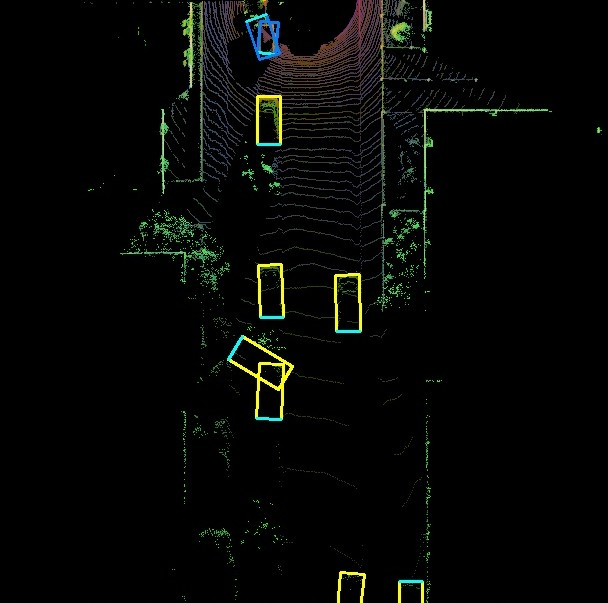
\includegraphics[width=\textwidth]{figures/000047.jpg}
    \caption{Float32 GPU Output}
\end{subfigure}
\hfill
\begin{subfigure}[b]{0.48\textwidth}
    \centering
    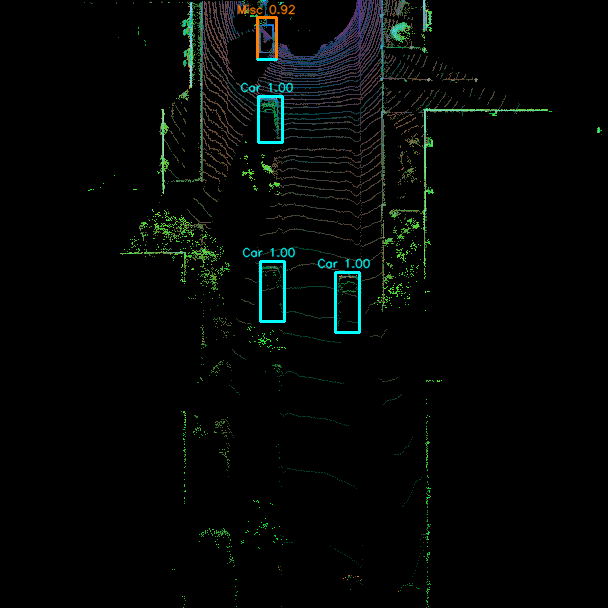
\includegraphics[width=\textwidth]{figures/bev_000047_det.png}
    \caption{INT8 FPGA Output}
\end{subfigure}
\caption{Comparison of Software (GPU) vs.\ Hardware (FPGA) detection results. Note the missing detections for distant objects in the hardware output.}
\label{fig:soft_vs_hard}
\end{figure}
The mechanism behind this accuracy drop is as follows:

\begin{itemize}[nosep]
    \item Distant objects produce very small activation values in the early convolutional layers ($<0.02$ in float32).
    \item INT8 quantization maps the full dynamic range to only 256 discrete levels ($-128$ to $+127$).
    \item The quantizer sets scaling factors to accommodate the majority of activations (dominated by nearby, high-signal objects).
    \item Small activations for distant objects are \textit{rounded to zero}, causing the signal to vanish entirely in the feature maps.
    \item Lowering the confidence threshold does not recover these detections because the signal is erased at the convolution stage, not at the decode stage.
\end{itemize}

This accuracy--efficiency trade-off is inherent to INT8 edge deployment and can be mitigated through Quantization-Aware Training (QAT) or mixed-precision strategies, as discussed in the future work section.

\section{Hardware Utilization Report}

Table~\ref{tab:hw_report} presents the hardware utilization report captured from the ZCU104 board during Complex-YOLOv4 inference.

\begin{table}[H]
\centering
\caption{ZCU104 Hardware Utilization Report During Inference}
\label{tab:hw_report}
\begin{tabular}{@{}p{4.5cm} p{9cm}@{}}
\toprule
\textbf{Metric} & \textbf{Measured Value} \\
\midrule
System RAM Usage & 613.0\,MB / 1985.5\,MB (30.9\% utilization) \\
Board Power (INA226) & 14,950\,mW ($\approx$15\,W) \\
DPU LUTs & $\sim$86,000 / 230,400 (37.3\%) \\
DPU Flip-Flops & $\sim$172,000 / 460,800 (37.3\%) \\
DPU BRAM & $\sim$270 / 312 (86.5\%) \\
DPU DSP Slices & $\sim$900 / 1,728 (52.1\%) \\
DPU Inference (per frame) & 140.1\,ms \\
\bottomrule
\end{tabular}
\end{table}

\textbf{Key Observation:} The BRAM utilization is 86.5\%, indicating that the DPU B4096 configuration nearly saturates the on-chip memory of the XCZU7EV device. This is expected, as BRAM is used to cache neural network weights and intermediate activations to minimize DDR4 access latency.


% ═════════════════════════════════════════════════════════════════════
%  CHAPTER 5: CONCLUSIONS
% ═════════════════════════════════════════════════════════════════════
\chapter{Conclusions}

This project successfully demonstrated the end-to-end deployment of two fundamentally different LiDAR-based 3D object detection architectures---Complex-YOLOv4 and SECOND---on the Xilinx ZCU104 FPGA platform. The key conclusions are:

\begin{enumerate}
    \item \textbf{Feasibility of FPGA Deployment:} Both models were successfully quantized to INT8, compiled to DPU-executable xmodels, and deployed on the ZCU104 board, confirming that FPGA-based edge inference is viable for autonomous driving perception.

    \item \textbf{Heterogeneous Compute Strategy:} The DPU accelerates standard dense operations (Conv2D, BatchNorm, ReLU, pooling). Architecturally complex or unsupported operations (such as YOLO decode and NMS) execute on the ARM CPU, while unsupported 3D sparse convolutions were bypassed using pre-computed inputs. This partitioning maximizes hardware utilization for the DPU-supported stages.
    
    \item \textbf{Complex-YOLOv4 Performance:} The 2D BEV model achieved 7.1\,FPS at $\sim$15\,W power consumption, demonstrating real-time-capable inference on an edge device with $10\times$--$20\times$ lower power than GPU alternatives.

    \item \textbf{SECOND Performance Analysis:} The 3D voxel model achieved $\sim$0.89\,FPS. Even with the sparse 3D convolutions pre-computed off-board, the ARM CPU became a severe bottleneck just from file I/O and anchor decoding. This profiling mathematically proves the necessity of developing custom hardware accelerators to bypass the CPU limitations.

    \item \textbf{Accuracy--Efficiency Trade-off:} INT8 quantization introduces a slight accuracy degradation, particularly for distant objects with small activation magnitudes. This is an inherent trade-off of fixed-point edge deployment.
\end{enumerate}

\section{Future Work}

The current deployment leverages the pre-designed DPU IP core, which is a general-purpose neural network accelerator with a fixed instruction set. While this approach provides rapid deployment and proven reliability, it has inherent limitations:

\begin{itemize}[nosep]
    \item The DPU cannot accelerate 3D sparse convolutions (critical for SECOND).
    \item The DPU cannot accelerate custom activation functions (Mish, SiLU).
    \item The fixed B4096 architecture may not optimally utilize the FPGA resources for a specific model.
\end{itemize}

The logical next step is the design of \textbf{custom HLS-based hardware accelerators} tailored to each model's specific computational patterns:

\begin{enumerate}

    \item \textbf{Custom Accelerator for Complex-YOLOv4:} A dedicated Darknet inference engine optimized for the specific layer sequence, residual connections, and route/concatenation patterns of the Complex-YOLOv4 backbone.

    \item \textbf{Sparse 3D Convolution Accelerator:} A hardware engine for the SECOND 3D sparse backbone, potentially using coordinate-based hash maps in on-chip memory to achieve FPGA-native sparse convolution without CPU involvement.

    \item \textbf{Quantization-Aware Training (QAT):} Retraining both models with simulated INT8 rounding to recover the accuracy lost for distant objects during PTQ.

    \item \textbf{Mixed-Precision Inference:} Running the first and last layers in INT16/FP16 to preserve small activation values for distant objects, while keeping the bulk of computation in INT8.
\end{enumerate}

The transition from the standard DPU to custom accelerators follows sound engineering methodology: \textit{first validate the model and pipeline end-to-end using the proven DPU infrastructure, then optimize with custom hardware once functional correctness is confirmed}. This staged approach ensures that any accuracy or performance issues observed on the board can be attributed to quantization or decode logic rather than hardware design errors.


% ═════════════════════════════════════════════════════════════════════
%  REFERENCES
% ═════════════════════════════════════════════════════════════════════
\bibliographystyle{IEEEtran}
\bibliography{references}


% ═════════════════════════════════════════════════════════════════════
%  APPENDICES
% ═════════════════════════════════════════════════════════════════════
\appendix

\chapter{Board Setup Commands}

\begin{lstlisting}[language=bash, caption={Transferring files to the ZCU104 board}]
# Copy xmodel to board
scp complex_yolov4_qat.xmodel root@<BOARD_IP>:/home/root/

# Copy test images
scp -r bev_images_test/ root@<BOARD_IP>:/home/root/

# Copy inference script
scp run_on_board.py root@<BOARD_IP>:/home/root/
\end{lstlisting}

\begin{lstlisting}[language=bash, caption={Running inference on the ZCU104}]
# Complex-YOLOv4 inference
python3 run_on_board.py --xmodel complex_yolov4_qat.xmodel \
    --image bev_images_test/bev_000001.npy \
    --conf 0.3 --save_img

# Hardware profiling
python3 run_on_board_profile.py --xmodel complex_yolov4_qat.xmodel \
    --image bev_images_test/bev_000001.npy --conf 0.3
\end{lstlisting}


\chapter{DPU Subgraph Analysis}

The compiled \texttt{.xmodel} for Complex-YOLOv4 contains 5 subgraphs, as revealed by the \texttt{xir.Graph} API:

\begin{lstlisting}[language=Python, caption={DPU subgraph inspection output}]
[0] device=USER  name=subgraph_DarknetBackbone__input_0
[1] device=DPU   name=subgraph_DarknetBackbone__MaxPool2d_...
[2] device=CPU   name=subgraph_..._conv110  (Head 2: 19x19)
[3] device=CPU   name=subgraph_..._conv102  (Head 1: 38x38)
[4] device=CPU   name=subgraph_..._conv94   (Head 0: 76x76)
\end{lstlisting}

This confirms that:
\begin{itemize}[nosep]
    \item \textbf{1 DPU subgraph} executes the entire Darknet backbone (from input through all conv/shortcut/route layers up to the three branch points).
    \item \textbf{3 CPU subgraphs} execute the final $1\times1$ convolutions that produce the 45-channel detection tensors for each YOLO head.
    \item \textbf{1 USER subgraph} handles the input preprocessing (format conversion).
\end{itemize}

The CPU-side execution of the final convolutions is a Vitis AI compiler decision based on the output tensor shapes and the DPU's output channel alignment requirements.


\chapter{Hardware Utilization Report --- Raw Output}

\begin{lstlisting}[caption={Complete hardware report from ZCU104 during Complex-YOLOv4 inference}]
============================================================
 HARDWARE UTILIZATION & PROFILING REPORT
============================================================

[1] Memory Utilization:
    System RAM : 613.0 MB used / 1985.5 MB total (30.9%)

[2] Power Consumption (INA226 Sensors):
    ina226 : 14950.0 mW

[3] DPU Hardware Utilization (ZCU104 B4096 overlay):
    Standard B4096 DPU (DPUCZDX8G) on ZCU104 requires:
      - LUTs : ~ 86,000
      - FFs  : ~172,000
      - BRAM : ~    270
      - DSPs : ~    900
============================================================
\end{lstlisting}

\end{document}
